\chapter{La réalisation du \appname et de la \platformename}
\phantomsection
\addcontentsline{toc}{section}{Introduction}
\section*{Introduction}

Dans ce chapitre, nous introduisons l'implémentation de notre projet. D'abord, nous
citons les différents langages programmation et les bibliothèques que nous avons manipulé.
Ensuite, nous présentons le \appname en détaillant ses fonctionnalités. Enfin, nous passons
à décrire la grande \platformename qui regroupe plusieurs programmes reliés aux théories de
l'incertain. Nous allons aussi expliquer comment cette platforme interagit avec ces programmes.

\section{Les langages de programmation et les bibliothèques utilisées}

Nous avons programmé l'interface du \appname en \textbf{Python 3}
en utilisant la bibliothèque \textbf{PyQt4}. Nous avons également réalisé la \platformename
avec \textbf{Java Swing}. De plus, plusieurs scriptes utilisés par cette
plateforme sont écrits en \textbf{MATLAB}. D'autres outils sont programmés en language
\textbf{C} et compilés sous une forme exécutable. Il y a aussi quelques programmes
qui nécessitent la présence de l'environement \textbf{Cygwin}.

\section{\appName}

Ce logiciel est constitué de deux parties, le noyau et l'interface graphique.
Il peut fonctionner sur tous les systèmes d'exploitation majeurs comme \textbf{Windows},
\textbf{\mbox{Mac OS X}}, \textbf{\mbox{GNU/Linux}} et \textbf{BSD}.

Le noyau est responsable d'effectuer les calculs après la lecture d'un fichier XML
contenant les données nécessaires pour l'application de la théorie de Dempster-Shafer.
Les résultats seront écrits dans un autre fichier XML. L'utilisateur n'a pas besoin
de comprendre la structure de ces fichiers, il lui suffit d'utiliser l'interface
graphique.

Cette interface est composée d'une barre de menu et de trois parties, les états
du monde, les hypothèses, et les agents. La barre contient les fonctionnalités principales
pour enregister, ouvrir, réinitialiser le projet et fermer l'application dans le menu
\textbf{Fichier}. Dans le menu \textbf{Projet}, on trouve les actions liées à la manipulation
du projet courant. On peut y changer le titre et donner une description au projet.\\[1em]

\begin{figure}[H]
\begin{subfigure}{0.49\textwidth}
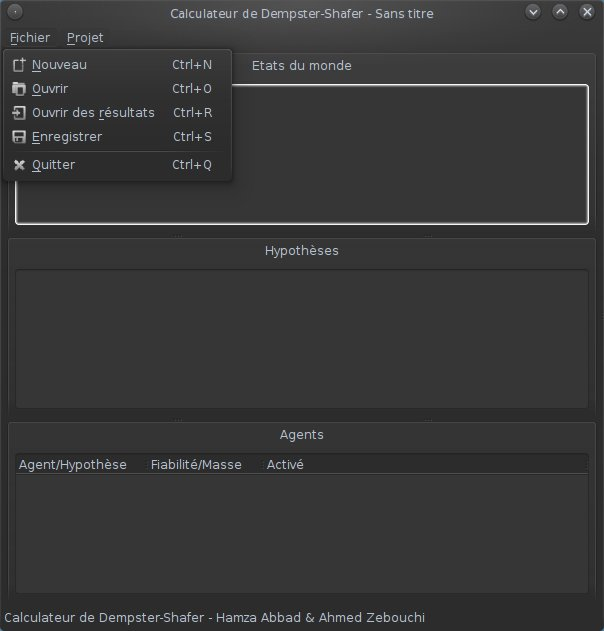
\includegraphics[width=\textwidth]{Inetrface_principale_menu_fichier}
\caption{Le menu \textbf{Fichier}}
\end{subfigure}
\hfill
\begin{subfigure}{0.49\textwidth}
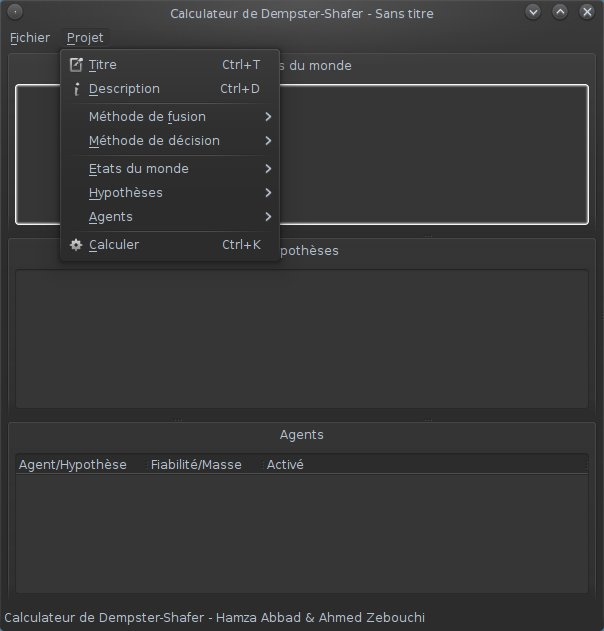
\includegraphics[width=\textwidth]{Inetrface_principale_menu_projet}
\caption{Le menu \textbf{Projet}}
\end{subfigure}
\caption{L'interface principale du \appname}
\end{figure}

Les états du monde, les hypothèses et les agents doivent s'ajouter dans cet ordre à partir
de ce menu ou par un clic droit dans leurs champs. \`A partir de ce menu, on peut choisir une
des méthodes de fusion: \textit{Dempster-Shafer}, \textit{Dubois-Prade}, \textit{Smets} ou
\textit{Yager}. On peut aussi choisir la méthode de décision qui sera utilisée parmi les trois
suivantes: \textit{Optimiste}, \textit{Pessimiste} ou \textit{Pignistique}.

On commence par ajouter tous les états du monde. Ensuite, chaque fois qu'on sélectionne certains
états, on établit une hypothèse à partir de ces états.\\[1em]

\begin{figure}[H]
\begin{subfigure}{0.49\textwidth}
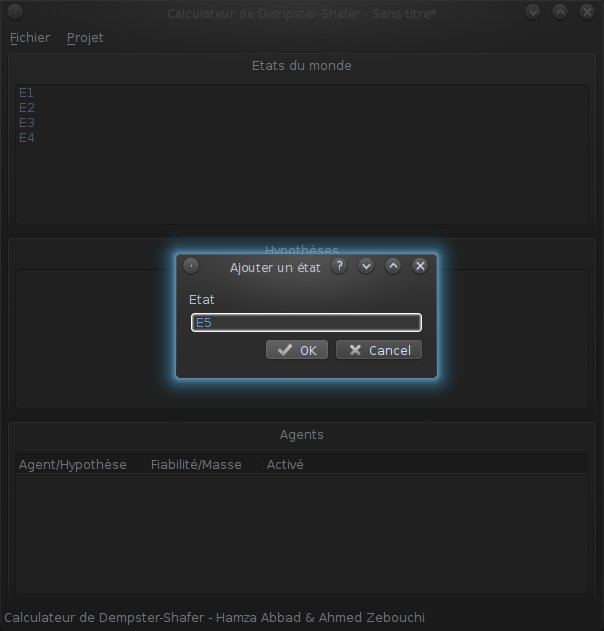
\includegraphics[width=\textwidth]{ajouter_etat}
\caption{Ajouter les états du monde}
\end{subfigure}
\hfill
\begin{subfigure}{0.49\textwidth}
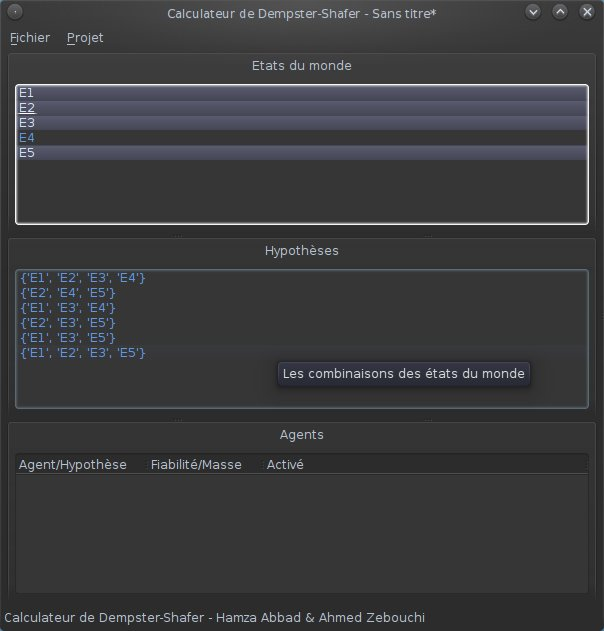
\includegraphics[width=\textwidth]{ajouter_hypothese}
\caption{Ajouter une hypothèse à partir des états}
\end{subfigure}
\caption{L'ajout des états du monde et les hypothèses}
\end{figure}

Par la suite, on doit procéder à l'ajout des agents. Chaque agent doit avoir un nom, un niveau de
fiabilité et un ensemble d'hypothèses tels que à chaque hypothèse est affectée une masse entre
$0$ et $1$.\\[1em]

\begin{figure}[H]
\begin{subfigure}{0.49\textwidth}
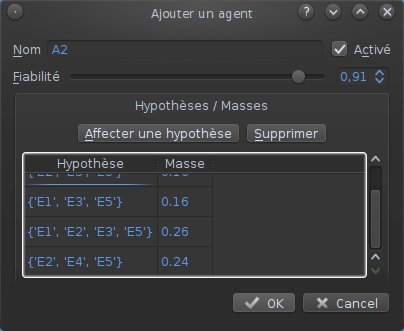
\includegraphics[width=\textwidth]{ajouter_agent}
\caption{Dialogue de l'ajout d'un agent}
\end{subfigure}
\hfill
\begin{subfigure}{0.49\textwidth}
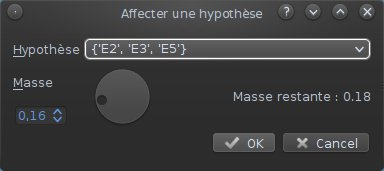
\includegraphics[width=\textwidth]{affecter_masse}
\caption{Dialogue de l'affectation d'une hypothèse}
\end{subfigure}
\caption{L'ajout d'un agent et l'affectation de ses hypothèses}
\end{figure}

Avant de passer au calcul, on doit enregistrer ces données dans un fichier à l'aide de la fonctionnalité
\textbf{Enregistrer} ou \textbf{Enregistrer sous}. Il faut aussi choisir un nom et un emplacement pour le
fichier. Il aura par défaut l'extention \texttt{.dsti.xml}. Cette action est nécessaire car elle génère
le fichier d'entrée pour le noyau. Si on ignore cette étape le programme demandera de la faire avant qu'on
puisse continuer.\\[1em]

\begin{figure}[H]
\centering
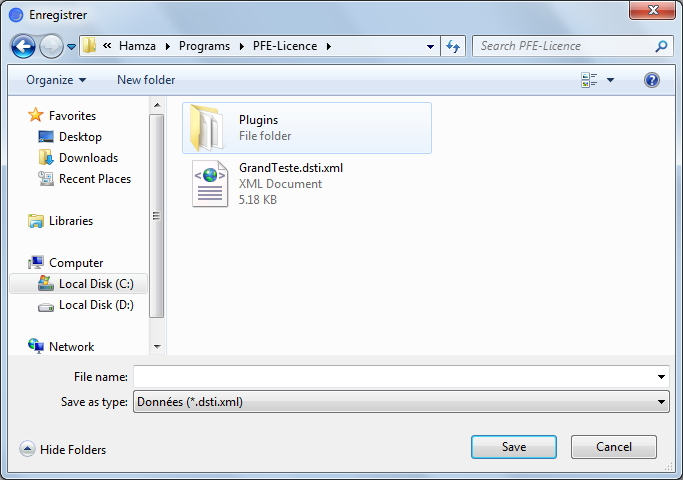
\includegraphics[width=0.8\textwidth]{Enregistrer}
\caption{Enregistrer les données}
\end{figure}

Enfin, on peut lancer le calcul. Cette étape risque de prendre un temps important si le nombre des états
du monde et/ou des agents est assez grand. Pour cela, un dialogue d'attente est affiché pendant l'exécution
du noyau en arrière-plan. L'utilisateur peut annuler cette opération à tout moment en cliquant sur le bouton
\emph{Annuler}.

Quand le calcul se termine, un dialogue contenant les informations du projet et tous les résultats sera affiché.
Les résultats sont obtenus par la lecture du fichier généré par le noyau qui a le même chemin que le fichier
sauvegardé, sauf qu'il porte l'extention \texttt{.dsto.xml}. Ce dialogue permet de rechercher une hypothèse en
tapant une partie de son nom dans la zone de texte qui contient le mot \emph{Rechercher}.
Les hypothèses qui correspondent à l'entrée de l'utilisateur sont sélectionnées afin de faciliter
la recherche. Il y a aussi un bouton permettant de créer un nouvel agent et de remplir ses hypothèses et ses masses
à partir de celles affichées. L'utilisateur doit introduire le nom de cet agent.

\begin{figure}[H]
\begin{subfigure}{0.39\textwidth}
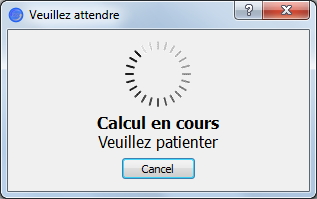
\includegraphics[width=\textwidth]{Dialogue_attente}
\caption{Dialogue d'attente}
\end{subfigure}
\hfill
\begin{subfigure}{0.59\textwidth}
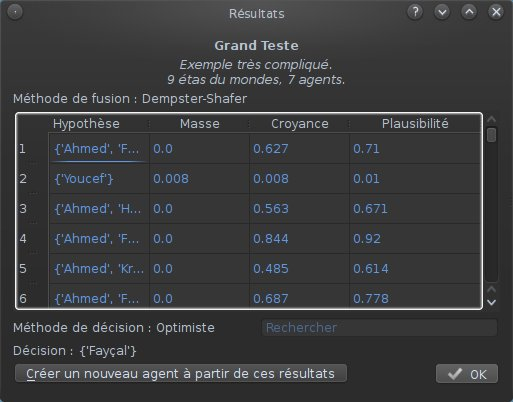
\includegraphics[width=\textwidth]{Dialogue_resultats}
\caption{Dialogue des résultats}
\end{subfigure}
\caption{Le calcul et l'affichage des résultats}
\end{figure}

Plus tard, on peut ouvrir les fichiers de données en utilisant l'action \textbf{Ouvrir} à partir du menu fichier. On
peut aussi afficher les résultats en ouvrant le fichier correspondant en utilisant l'action \textbf{Ouvrir des résultats}.

\begin{figure}[H]
\begin{subfigure}{0.49\textwidth}
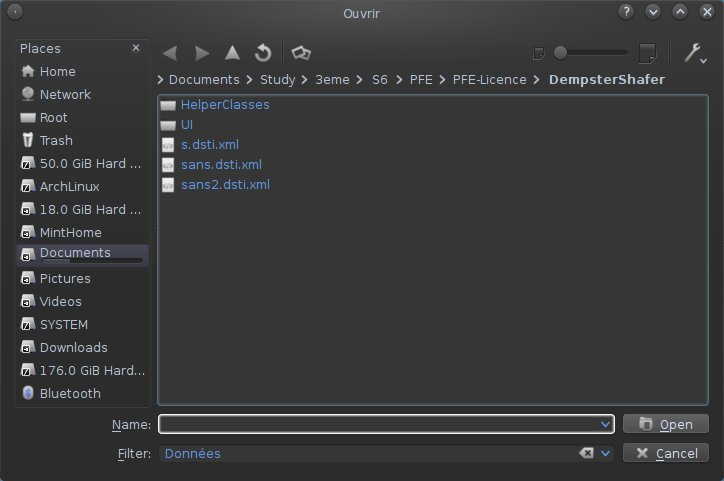
\includegraphics[width=\textwidth]{Ouvrir}
\caption{Dialogue d'ouverture d'un fichier de données}
\end{subfigure}
\hfill
\begin{subfigure}{0.49\textwidth}
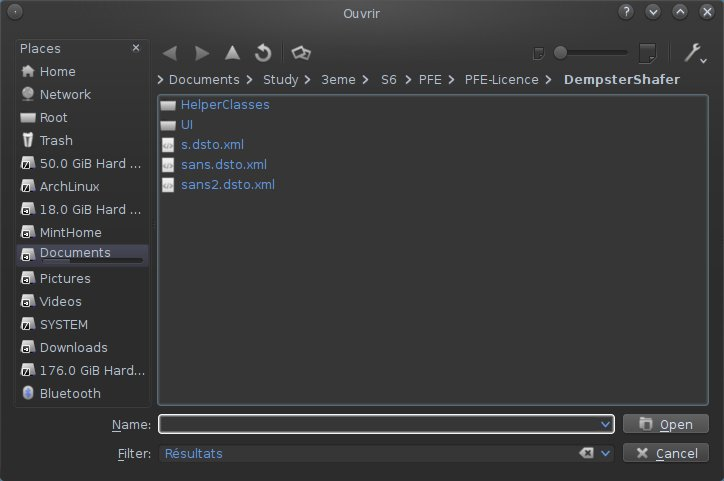
\includegraphics[width=\textwidth]{Ouvrir_resultats}
\caption{Dialogue d'ouverture de résultats}
\end{subfigure}
\caption{Les dialogues de l'ouverture d'un fichier}
\end{figure}

\section{\platformeName}

Ce programme est une interface composée de plusieurs panneaux et chaque panneau est accessible
à partir de son titre dans la barre des onglets. Un panneau comporte une ou plusieurs interfaces pour
un ou plus d'un programme externe.  La \platformename est facilement extensible; pour ajouter un nouveau
panneau dans cette interface il suffit de créer une classe personnalisée qui dérive de la classe
\mbox{\texttt{javax.swing.JPanel}} dans le paquet \texttt{Plugins}. Jusqu'à présent, la \platformename
contient quatre onglets : \textit{Imprécision}, \textit{Décision}, \textit{Incertain}
et \textit{Tools}.

Dans le panneau \textit{Imprécision} il y a un bouton pour lancer la \textbf{Fuzzy Logic Toolbox} qui est une
bibliothèque de \textit{MATLAB} avec une interface graphique intégrée facilitant l'exploitation directe
de la bibliothèque.

\begin{figure}[H]
\centering
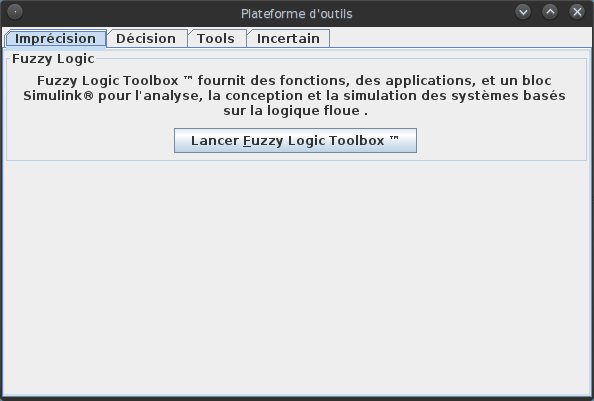
\includegraphics[width=0.7\textwidth]{Imprecision}
\caption{Le panneau \textbf{Imprécision}}
\end{figure}

Le panneau \textit{Décision} contient deux parties, une qui s'appelle \textit{Logique}
contenant un bouton pour exécuter l'application \textbf{DecPos} qui permet d'effectuer des calculs sur la
décision et d'autres opérations sur les bases possibilistes, et l'autre qui s'appelle \textit{Graphique} pour
exécuter \ldots.
\newsavebox{\screenshot}
\begin{figure}[H]
\begin{subfigure}{0.49\textwidth}
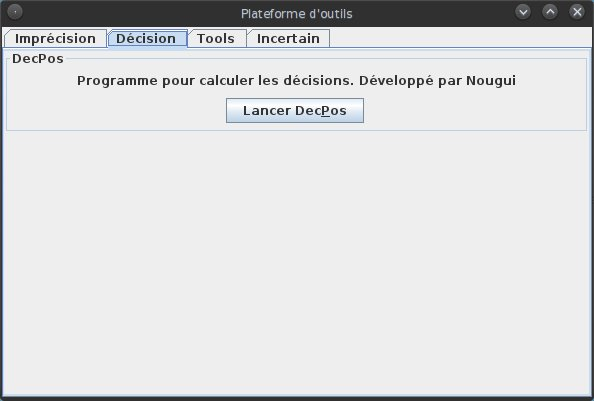
\includegraphics[width=\textwidth]{Decision}
\caption{La partie \textbf{Logique}}
\end{subfigure}
\hfill
\begin{subfigure}{0.49\textwidth}
\fbox{\parbox[t][5.1cm][t]{\textwidth}{\hfill}}
\caption{La partie \textbf{Graphique}}
\end{subfigure}
\caption{Le panneau \textbf{Décision}}
\end{figure}

Dans le panneau \textit{Incertain}, on trouve les interfaces nécessaires pour dessiner un graphe orienté sans
cycles de nature BNT ou PNT et pour modifier ses paramètres après la validation. Ces interfaces permettent de générer
un script \textit{MATLAB} et de l'exécuter.

\begin{figure}[H]
\centering
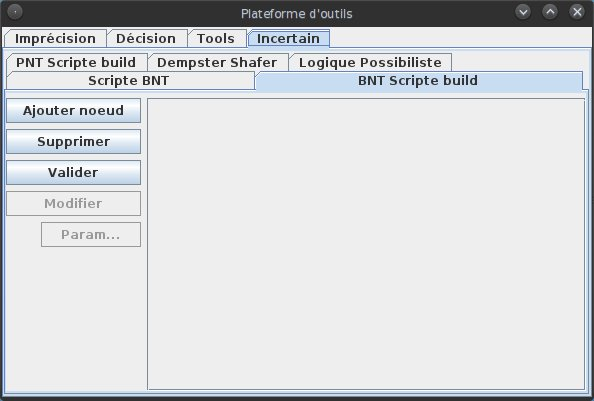
\includegraphics[width=0.7\textwidth]{Incertain_BNT_graphe}
\caption{L'interface du graphe BNT}
\end{figure}

Dans le même panneau, il y a aussi un panneau interne qui porte le nom \textit{Dempster-Shafer} pour exécuter
notre application \appname qui a été expliquée auparavant. Le dernier panneau est ce de la \textit{Logique possibiliste}.
Il représente une interface pour un ensemble des programmes qui seront exécutés en série. Il permet de spécifier le nombre
de noeuds dans un graphe possibiliste et le nombre maximal de parents pour chaque noeud, ainsi que le nombre de propositions
(1 ou 2). Le programme génère un graphe aléatoire par lancer un script \textit{MATLAB} suivi par deux programmes
\texttt{passage} et \texttt{inference}. Enfin, il affiche les résultats pour l'utilisateur.

\begin{figure}[H]
\begin{subfigure}{0.49\textwidth}
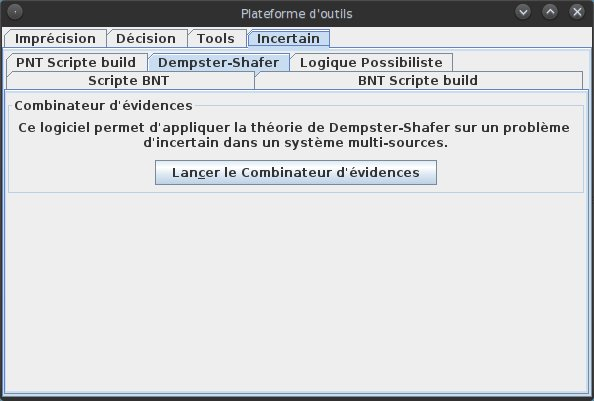
\includegraphics[width=\textwidth]{Incertain_DS}
\caption{Le panneau interne \textbf{Dempster-Shafer}}
\end{subfigure}
\begin{subfigure}{0.49\textwidth}
\hfill
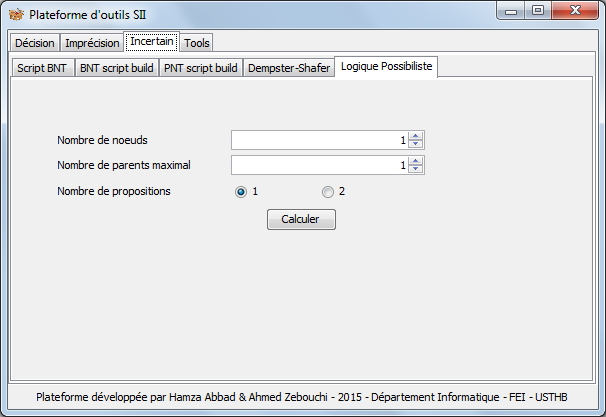
\includegraphics[width=\textwidth]{Incertain_LP}
\caption{Le panneau interne \textbf{Logique possibiliste}}
\end{subfigure}
\caption{Le panneau \textbf{Incertain}}
\end{figure}

Il reste le panneau \textit{Tools} qui contient deux interfaces pour utiliser le logiciel \textbf{UBCSAT}, la
première pour calculer le SAT et la deuxième pour le Weighted Max SAT. L'utilisateur doit introduire les formules
logiques FND\footnote{Forme normale disjonctive}.

\begin{figure}[H]
\centering
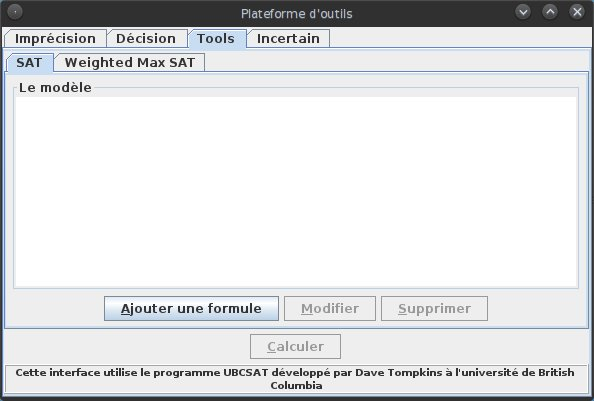
\includegraphics[width=0.7\textwidth]{Tools_SAT}
\caption{Le panneau \textbf{Tools}}
\end{figure}

\phantomsection
\addcontentsline{toc}{section}{Conclusion}
\section*{Conclusion}

Nous avons présenter globalement ce que nous avons réalisé dans notre projet. Nous avons commencé par une
présentation détaillée de notre application \appname que nous avons entièrement développé, et puis, nous
avons montré les différentes tâches qui peuvent être réalisées à travers notre interface \platformename.